\section{Convolutional Neural Networks}

\subsection{Theory}

\begin{enumerate}
    \item  The output volume is:
    
    \begin{align*}
        \ldots
    \end{align*}
    \item Including bias parameters, this hidden layer has the following number of parameters:
    
    \begin{align*}
        \ldots
    \end{align*}    
    \item The output from the simple convolutional layer for the given filter and input is:
    
        \begin{table}[H]
        \centering
        \begin{tabular}{ |c|c|c|c| } 
         \hline
         \textbf{Row} &  \textbf{Column} &  \textbf{Filter} & \textbf{Value} \\
         \hline
         1 & 1 & 1 & ---\\
         1 & 1 & 2 & ---\\
         1 & 2 & 1 & ---\\
         2 & 1 & 1 & ---\\
         \hline
        \end{tabular}
        \caption{Output from convolution}
        \label{cnnValTable}
        \end{table}
    \item The total number of trainable parameters in this network is:
    \begin{align*}
        \ldots
    \end{align*}  

    \item State two advantages of convolutional neural networks over fully connected networks.
    
    $\ldots$
\end{enumerate}

\subsection{Programming}
For this question, refer to the Jupyter Notebook. You will be using PyTorch to implement a convolutional neural network -- the notebook will have detailed instructions. We will be using the fashion MNIST dataset for a classification task.

\subsubsection{Convolutional Neural Network}
Add the accuracy and the loss curve from tensorboard in this report:

\begin{figure}[H]
    \centering
    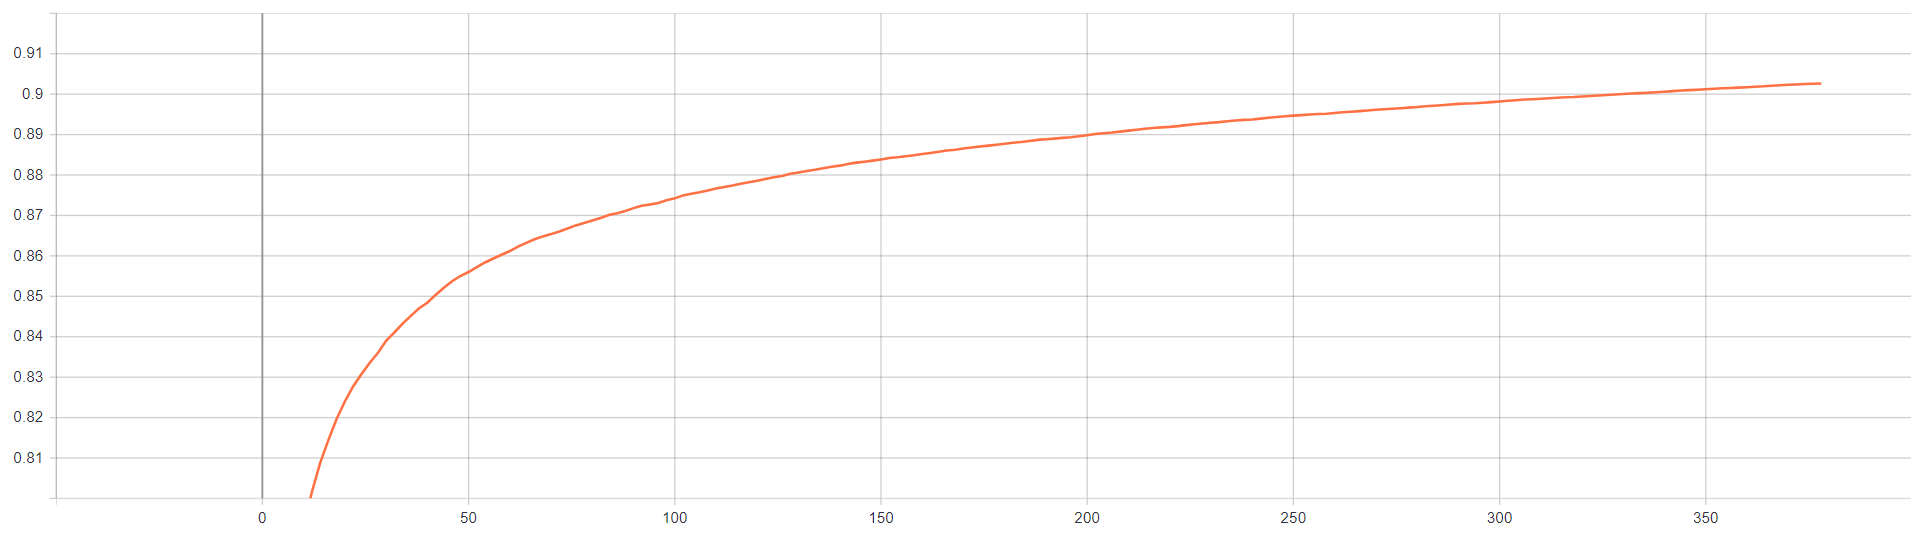
\includegraphics[width=1.0\textwidth]{templates/accuracy}
    \caption{Accuracy curve}
    \label{fig:acc_curve}
\end{figure}

\begin{figure}[H]
    \centering
    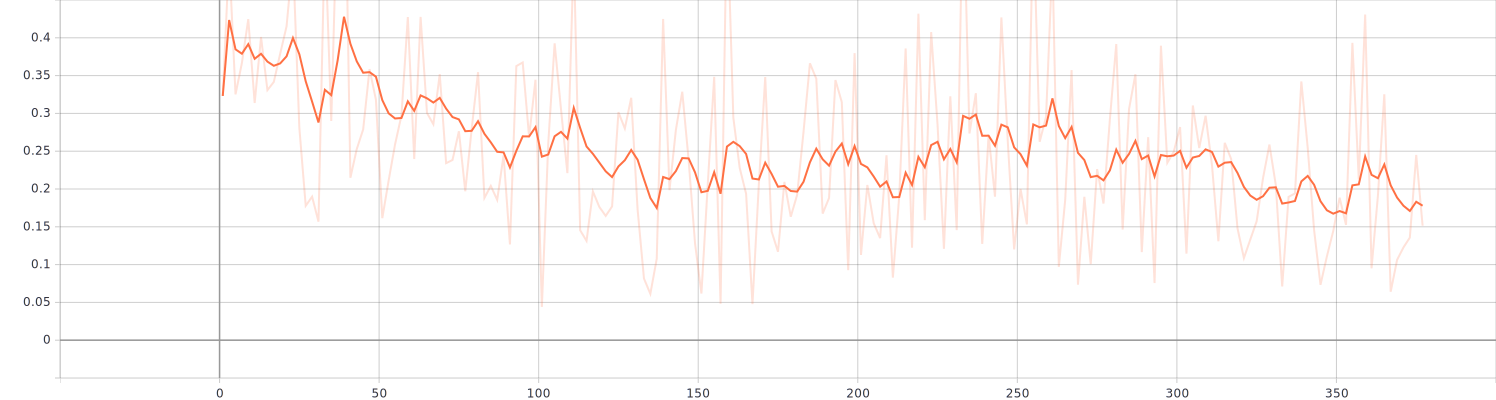
\includegraphics[width=1.0\textwidth]{templates/loss}
    \caption{Loss curve}
    \label{fig:loss_curve}
\end{figure}

\subsubsection{Accuracy}
 Report the overall accuracy and the per-class accuracy:

We did not choose to make any improvements to the baseline model, hence do not need to provide an explanation of our model architecture.
\begin{table}[H]
\centering
\begin{tabular}{ |c|c| } 
 \hline
 Overall Accuracy & 89 \% \\
 \hline
\end{tabular}
\caption{Overall Accuracy for Convolutional Neural Network}
\label{nnOA}
\end{table}


\begin{table}[H]
\centering
\begin{tabular}{ |c|c| } 
 \hline
 \textbf{Class} & \textbf{Accuracy} \\
 \hline
 T-shirt/top & 88 \% \\
 Trouser & 99 \% \\
 Pullover & 85 \% \\
 Dress & 90 \% \\
 Coat & 82 \% \\
 Sandal & 96 \% \\
 Shirt & 74 \% \\
 Sneaker & 96 \% \\
 Bag & 98 \% \\
 Ankle boot & 96 \% \\
 \hline
\end{tabular}
\caption{Per Class Accuracy for Convolutional Neural Network}
\label{nnCA}
\end{table}

Identify the problematic classes and list the possible reasons as to why these classes may have significantly lower accuracy compared to other classes.

The problematic classes here were Shirt, Coat and T-Shirt / top. Some possible reasons why these classes have significantly lower accuracy compared to other classes:
\begin{itemize}
	\item A lot of t-shirts get classified as shirts and vice versa because of the similarities in visual appearance of the garments.
	\item Coats can also be wrongly classified as shirts, since both have collars and long sleeves.
\end{itemize}

To rectify this issue, we can perform data augmentation for these problematic classes to improve the classifiers performance.